\documentclass[american]{scrartcl}

    \newcommand{\lang}{en}

    \usepackage{babel}
    \usepackage[utf8]{inputenc} 
    \usepackage{csquotes}
    \usepackage{amsmath, amssymb}
    \usepackage{graphicx}
    \usepackage{tikz} 

    \setlength{\parindent}{0em}
    \setlength{\parskip}{0.5em}

    % Graphs
    \usetikzlibrary{positioning}
    \tikzset{main node/.style={circle, draw,minimum size=1cm,inner sep=3pt},}

    % Math commands
    \newcommand{\E}{\mathbb{E}}


    \usepackage[
        bibencoding=utf8, 
        style=apa
    ]{biblatex}

    \bibliography{../../../Desktop/bibliographies/thesis}
    
    
    \usepackage{amsmath}
    \title{
        Trophic Analysis of a Prosumer Electricity Market
    }

    \author{Andrea Titton}
    
\begin{document}

\nocite{*}
\maketitle

\section{Introduction}

In recent years the economy found itself in the midst of a strong and vital public push towards decarbonisation of the energy sector. One aspect of such process is the increased adoption by households of technology to produce electricity independently, like solar panels, batteries, and ``smart'' meters (\cite{Parag2016}).

In coming years, this change in the households' role in the energy market, from consumers to prosumers, will present policy makers and economists with a vast spectrum of opportunities and challenges. In particular, the transition from centralized and oligopolistic fossil fuel producers to distributed renewable energy prosumers calls for a shift in economic modelling of energy markets, both in methodology and objectives. A shift is needed in methodology because the network structure and heterogeneity of producers add fundamental non-linearities in the market clearing mechanism. With regards to objectives, questions of efficiency and resilience in models with complex networks cannot be addressed through a traditional homogenous policy, and therefore require understanding of the heterogenous dynamics within the market structure.

\section{Research Question}

The project's main objective will be to identify the conditions under which a decentralized prosumer market for electricity displays aggregate resilience.

The research question will be dealt with on three dependent levels. First, the resilience properties will be investigated within a theoretical framework. Second, based on the theoretical model, an empirical analysis will be formulated. Third, the empirical result will define suitable policy implications.

\section{Methodology}

\subsection{Notion of resilience}

The notion of network resilience will be mapped to three properties of dynamical systems.

First, systemic stability, which arises when a network's critical points are robust to perturbations of its nodes. For example, a desirable property for an electricity market of prosumers is its ability to prevent systematic shortages following a weather shock.

Second, self-organized criticality, as presented by \citeauthor{Bak1995} (\citeyear{Bak1995}), which concerns the ability of the system to evolve towards critical points with the same characteristics, regardless of the parameters and scale. In the context of our model, this implies that the pricing mechanism and equilibria of the proposed market should display scale-invariant characteristics.

Third, Lyapunov stability, which refers to the stability of a solution near the equilibrium. Applied to a prosumer electricity market, it is desirable for the equilibrium price vector of electricity to be stable around the market clearing price.

\subsection{Theoretical model}

The electricity market will be modeled as a two layers market. First, there is a local prosumers market with electricity endowments modeled as a random process. Furthermore prosumers can decide to trade electricity with a local firm who owns the electricity grid. The consumption and trading decision then determines the aggregate demand or supply of electricity by prosumers which the local firm has to face. The grid firm is modeled, in the second layer, as a node in a network of local firms, called hereafter backbone market. Each node is associated with a unique local market. This way, firms can trade with neighboring firms in order to sell excess supply of energy or meet excess demand generated by their local market.


Prosumers are assumed to be heterogenous, risk-averse agents with bounded rationality, making decisions in discrete time. Agents form expectations over the price dynamics via rules of thumb, updated in an evolutionary manner. The agents' behavior will be driven by a dynamic optimization problem in discrete time. In particular, the goal of each prosumer is to smooth its energy consumption at or around its necessity level.

Grid firms are also assumed to be heterogenous, with bounded rationality, and profit maximizing agents, making decisions in discrete time. The heterogeneity arises in characteristics of the local market they are located in. Firms make, as prosumers, decision based on rules of thumb forecasting and bargain prices with neighboring firms.

This heterogeneity allows for the model to display spatial herd behavior, that is, firms behaving similarly within network clusters. In particular, firms maximize profit given current backbone prices and expected local market price dynamics.

In economic models the market clears via an endogenous mechanism. The first mechanism to consider is a centralized energy price, either generated exogenously by the government under complete information or endogenously via an auction mechanism. A more interesting pricing mechanism worth considering is pairwise bargaining. In particular, the market clears via a vector of prices (one for each edge) that solves the bargaining problems between two nodes, derived as in \citeauthor{Bedayo2016} (\citeyear{Bedayo2016}).

\subsection{Graph properties}

Given the analysis' premises (i.e. the model) and objective (i.e. the dynamical properties that we associated to the concept of resilience), the focus will be on finding a concise way to map one to the other. Particular difficulties arise due to the high dimensionality of the parameter space and the non-linearities introduced by the network structure. One way to approach this problem is to rely on spectral graph theory.

Among the various spectral graph measures trophic analysis appears \textit{ex-ante} particularly suited for the task at hand. We will employ an analogous procedure to that of \citeauthor{MacKay2020} (\citeyear[p.~19]{MacKay2020}). The goal is to create a link between the model's structure and its dynamics by deriving a formula for the trophic levels and associated trophic incoherence value ($F_0$), defining a set of shocks the network could face, and then expressing the resilience to such shocks as a function of $F_0$.

Using trophic coherence as a pivot to the model's dynamics, as opposed to more traditional economic metrics such as upstreamness (\cite{Antrs2012}), offers three main advantages. First, it does not require ``source'' nodes in directed graphs, hence it is defined for cycle graphs. Second, it is robust to local computation, that is, assuming we can only observe or model a subgraph, the trophic levels are constant in the inner graph and do not vary drastically around truncations (\cite[p.~19]{MacKay2020}). Third, its interpretation is fundamentally linked to that of the \textit{spectral radius} of a graph, which regulates the behavior of most dynamical systems on graphs, despite being simpler to measure.

These three properties allow for an empirically and theoretically consistent, robust, and easily computable metric that acts as map to navigate the complex network dynamics.

\subsection{Empirical testability}

The calibration for the empirical analysis needs to estimate both agent specific characteristics, namely attitude towards risk and forecasting rule, as well as structural network characteristics, namely the number of prosumers and their respective possibility to trade.

The network structural characteristics can be estimated using existing datasets on energy markets, such as the \textit{Open Power System Data} (\cite{Wiese2019}), and data on prosumers networks. Given the data, one can construct the underlying graph and calibrate the model's parameters through electricity trade between prosumers.

The agent's characteristics can be estimated in a controlled lab setting via \textit{Learning to Forecast experiments} (adapted from \cite{Hommes2013}). The core method is to devise experiments in which participants are faced with simple dynamic optimization tasks, analogous to those faced by prosumers in our model, and estimating which rule of thumb forecasting method, out of a predetermined set, they use in which context.

\subsection{Policy implications}

The last step of the analysis will consist of testing various potential policies on the developed model. Of particular interest are dynamic policies, such as taxation or subsidies, and structural policies, such as constructing new edges (i.e. cables between distributors), which allow the system to converge to a more resilient system via the least disruptive path.

\section{Conclusion}

Prosumer energy markets are already a reality today and will become more ubiquitous as the decarbonisation of the economy enters more advanced stages. The diffused market structure and the fact that decision will be taken by prosumers, on top of firms, prevent us from relying on traditional economic modelling techniques to understand and shape the energy market transition.

Hence, building on energy policy considerations by \citeauthor{Parag2016} (\citeyear{Parag2016}), the aim is to construct and estimate a network model in discrete time with heterogenous and rationally bounded agents. The dynamical analysis will employ techniques from dynamical systems, such as the aforementioned stability concepts, and complex networks, in particular trophic analysis. These techniques are necessary in face of the strong non-linearities within the model.

The model will mainly be employed to ask questions around resilience and assess policies aimed at transitioning the market towards a stable configuration in a non-disruptive manner.

\newpage
\pagenumbering{gobble} % stop page numbering
\printbibliography

\newpage
\appendix

\section{Model}

\iffalse
    \subsection{Network structure}

    \centering
    \begin{tikzpicture}[->]
        % Nodes
        \node[main node] (1) {Local\\market};
        \node[main node] (2) [right = 2cm of 1] {Firm 1};
        \node[main node] (3) [right above = 2cm of 2] {Firm 2};

    \end{tikzpicture}
\fi

\subsection{Prosumers}

\subsubsection{Normal preferences}

The prosumer instantaneous utility of electricity consumption is,

\begin{equation*}
    u_i(x) = d_i \cdot \ln(x),
\end{equation*}

where $d_i$ is an heterogenous demand parameter.

Furthermore, agents get electricity endowment $e_{i, t}$ which follows a random exogenous process and have a given stock of cash-in-hand $m_t$, starting from $m_0$. Furthermore agents can buy or sell electricity $x_t$ at price $p_t$.

The dynamic optimization problem is then,

\begin{equation*}
    \begin{split}
        \pi_t(x_t \vert e_{i, t}) &= u_i(x_t + e_{i, t}) + \beta \cdot \E_t \left[ \pi_{t+1}(x_{t+1} \vert e_{i, t+1}) \right] \\
        s.t. \ \ m_{t+1} &= m_t - p_t \cdot x_t \text{ and } m_t \geq 0
    \end{split}
\end{equation*}

Hereafter we will suppress $i$ for convenience.

Agents are assumed to make forecasts over the price $p_{t+1}$, using a linear forecasting rule $\E_t[p_{t+1}] = \psi_{h, t} \cdot p_t$, where $\psi_h \in \Psi$ is selected in a manner similar to \citeauthor{Hommes2013} (\citeyear{Hommes2013}).

Using the budget constraint we can redefine the problem as,

\begin{equation}
    x_t = \frac{m_t - m_{t+1}}{p_t},
\end{equation}

such that the agents control variable is the next level of cash-in-hand $m_{t+1}$. This gives the Euler equation,

\begin{equation}
    u^\prime\left( e_t + \frac{m_t - m_{t+1}}{p_t} \right) = \beta \cdot \E_t \left[ u^\prime\left(e_{t+1} + \frac{m_{t+1} - m_{t+2}}{ \psi_{h, t} \cdot p_t} \right)  \right].
\end{equation}

The endogenous grid method can then be used to find a policy function

\begin{equation}
    m^\prime(m_t, p_t \ \vert \ \psi_{h, t}, e_t).
\end{equation}

The solution of the local problem yields the following electricity demand in a state of high endowments and different conditions $m_t$ (Figure \ref{fig:demand})

\begin{figure}[b]
    \caption{Electricity demand curve for an agent}
    \centering
    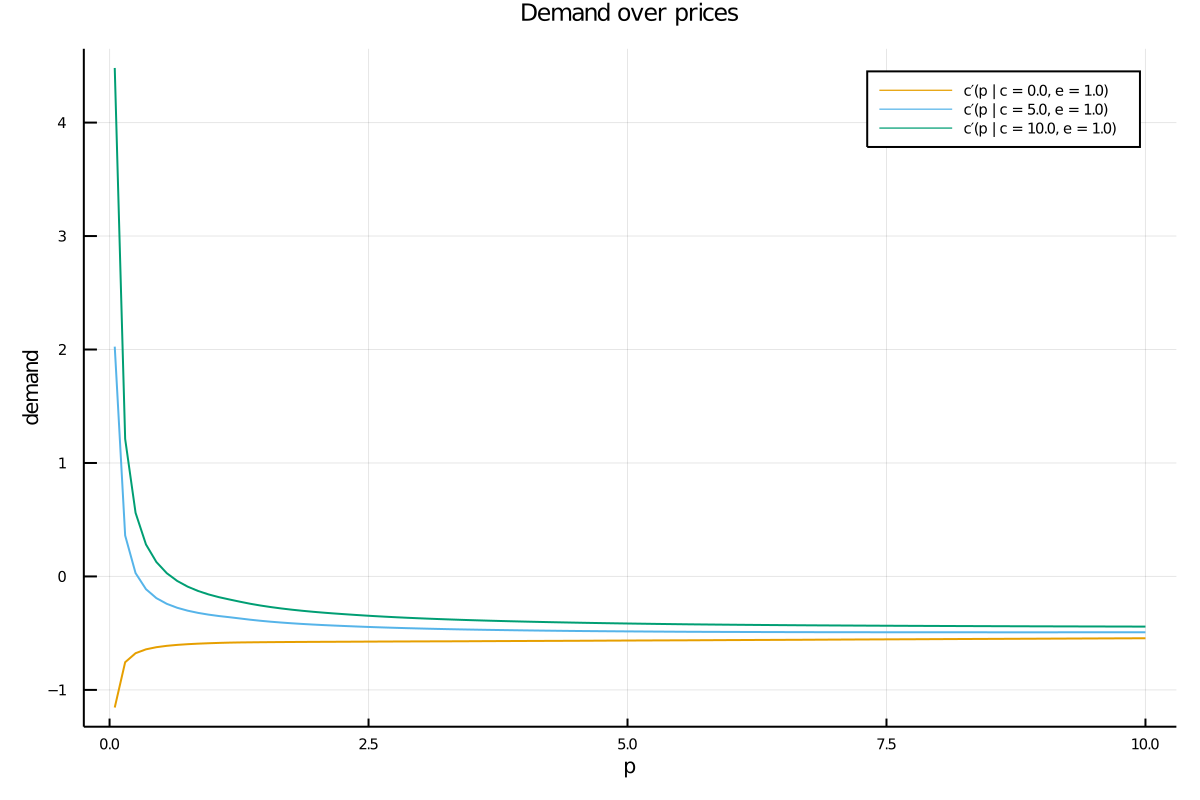
\includegraphics[width=0.9\textwidth]{../../plots/markets/pricedemand.png}
    \label{fig:demand}
\end{figure}

and the following simulation run (Figure \ref{fig:sim}).

\begin{figure}[b]
    \caption{Simulation of an agent with switching forecasting rule and $AR(1)$ price process}
    \centering
    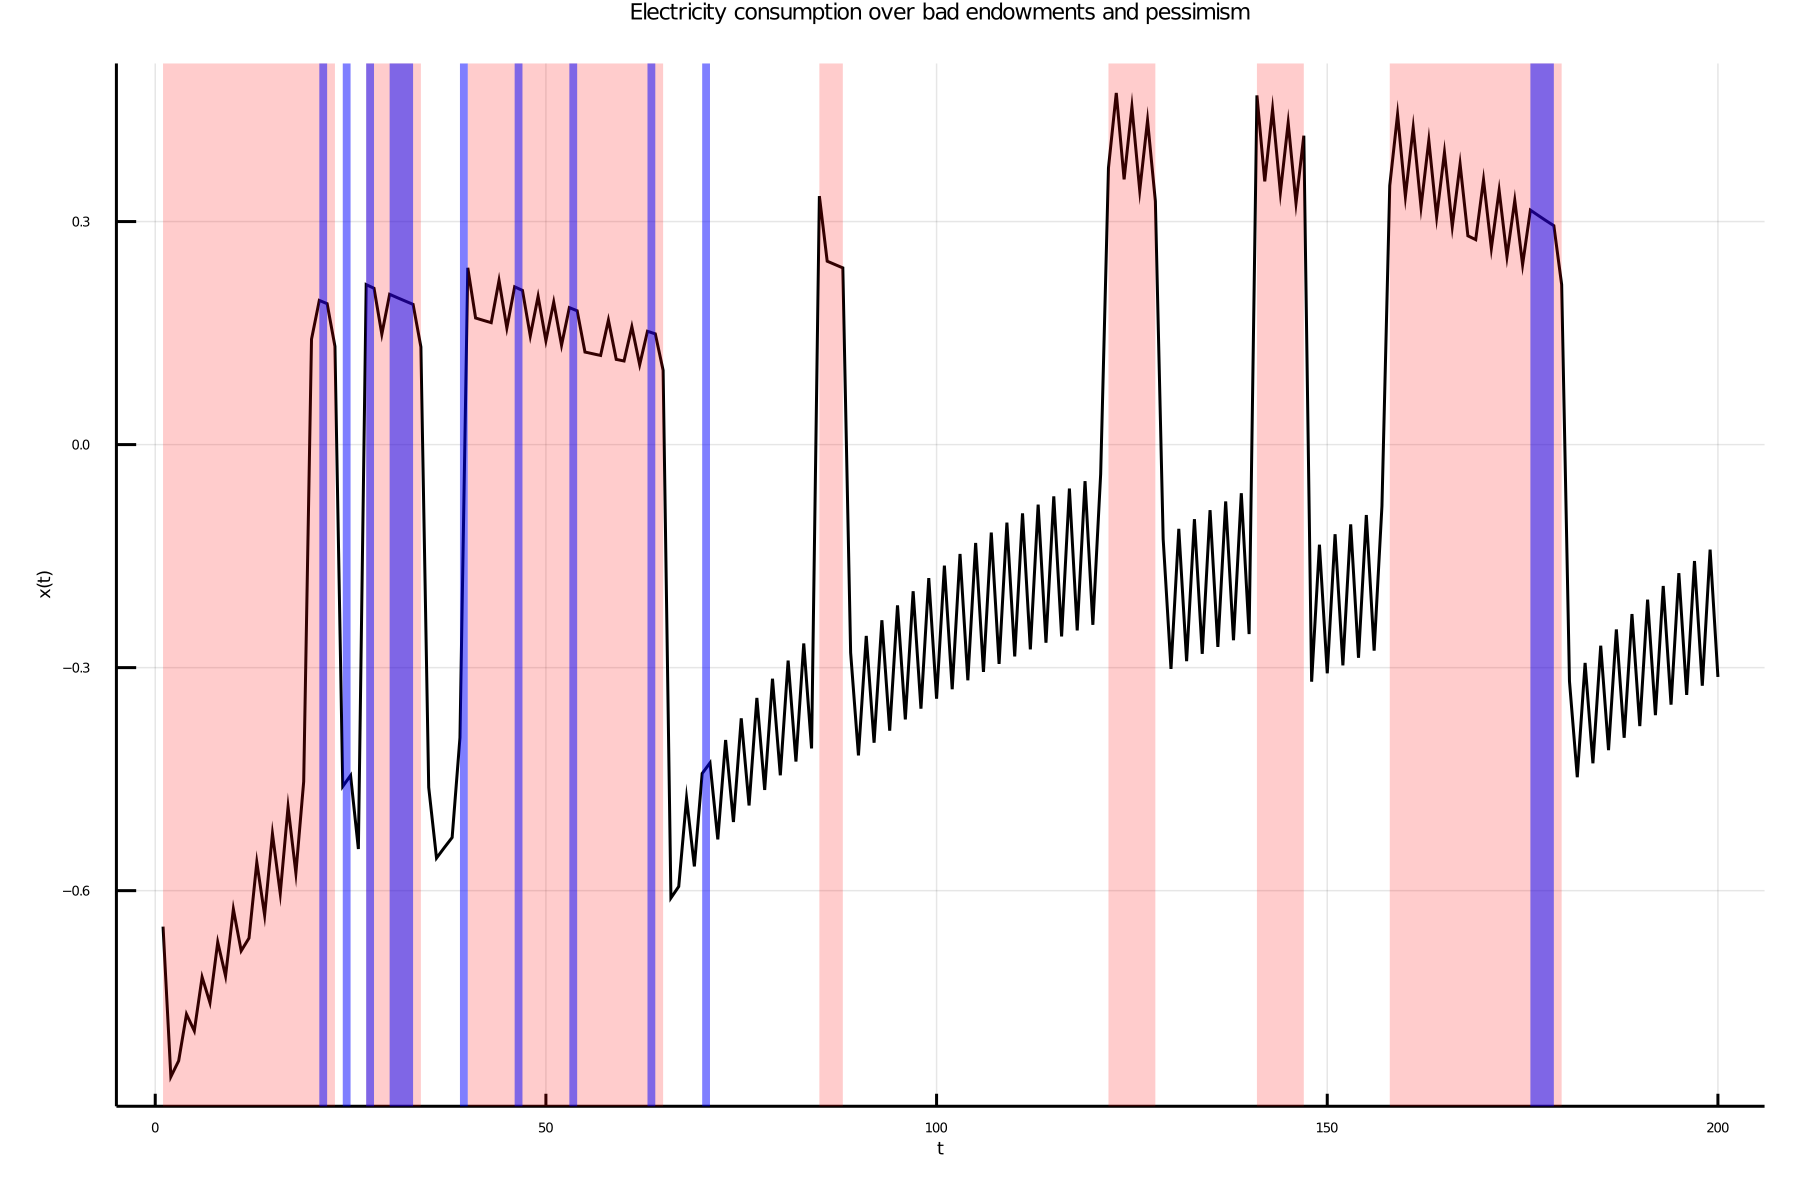
\includegraphics[width=0.9\textwidth]{../../plots/markets/simul.png}
    \label{fig:sim}
\end{figure}

\subsubsection{Epstein-Zin preferences}

A better formulation, using Epstein-Zin preferences,

\begin{equation}
    U_t = \left[ (1 - \beta) \cdot u(x_t)^{\frac{\phi - 1}{\phi}} + \beta \cdot \mu_t(U_{t+1})^{\frac{\phi - 1}{\phi}} \right]^{\frac{\phi}{\phi - 1}}
\end{equation}

where the certainty equivalent is,

\begin{equation}
    \mu_t(U) = \E_t\left[ U^{1 - \gamma} \right]^{\frac{1}{1 - \gamma}}.
\end{equation}

As Caldara, introduce,

\begin{equation}
    \theta := \frac{1 - \gamma}{1 - \frac{1}{\phi}}.
\end{equation}

\end{document}